\documentclass[12pt]{report}
%\documentclass[14pt]{extreport}
%documentclass[12pt]{book}
\usepackage{titlesec}
\usepackage{UVconfig}
%%%%%%%%%%%%%%%%%%%%%%%%%%%%%%%%%%%%%%%%%%%%%%%%%%%
% Permite usar los comandos \AU{texto} para dar color al texto. También para \Di{texto}. 
\usepackage{color}
\newcommand{\JP}[1]{\textcolor{blue}{[JP: #1]}}
\newcommand{\HL}[1]{\textcolor{red}{[HL: #1]}}
\newcommand{\CC}{\cellcolor{lightgray}}



%%%%%%%%%%%%%%%%%%%%%%%%%%%%%%%%%%%%%%%%%%%%%%%%%%%%%
%Use este espacio para agregar paquetes extra.

%%%%%%%%%%%%%%%%%%%%%%%%%%%%%%%%%%%%%%%%%%%%%%%%%%%%%%%
% Final del preambulo

%%%%%%%%%%%%%%%%%%%%%%%%%%%%%%%%%%%%%%%%%%%%%%%%%%%%%%%%%%
% Inicio del documento
\begin{document}


%Aquí va el tipo de documento
\renewcommand{\UVdoc}{}

%Aquí va su programa académico
\renewcommand{\UVprograma}{Programa Académico de Ingeniería Electrónica}

%Aquí va el título de su documento
\renewcommand{\UVtipo}{Informe técnico de proyecto de práctica profesional}
\renewcommand{\UVtitulo}{Implementación de una plataforma SIEM para el monitoreo, correlación y deteccion de eventos de seguridad en una infraestructura de un proveedor de servicios de telecomunicaciones}

% Aquí va su nombre. Si son varios, use la segunda opción
\renewcommand{\UVautor}{Camilo Home Buriticá} \tabularnewline 

\renewcommand{\UVempresa}{Empresas Municipales de Cali EICE ESP}
%\renewcommand{\UVautor}{Nombres y apellidos del autor1 \par %\vspace{-0.5cm} igual para el autor2 }

% Aquí va el nombre de su director. Si son varios, use la segunda opción
\renewcommand{\UVdireccion}{Director de programa}
\renewcommand{\UVdirector}{Andrés David Restrepo Girón \tabularnewline}

% \renewcommand{\UVdirector}{Director Nombre Apellido}

% Si existe, aquí va el nombre de su codirector. Si son varios, use la segunda opción
% En caso de no existir esta figura, use \renewcommand{\UVcodireccion}{} y \renewcommand{\UVcodirector}{} para que no aparezca en la portada.

%\renewcommand{\UVcodirector}{Martha Lucía Orozco Gutiérrez, Ph.D. \tabularnewline}%Diego Zuluaga, Ing. Exc. MBA}
%\renewcommand{\UVcodirector}{coDirector1 \tabularnewline & coDirector2 nombre y apellido}

%\renewcommand{\UVAsesoria}{Asesor:}
%\renewcommand{\UVAsesor}{Bayron Andres Calvache Vallejo, M.Sc.
%\tabularnewline}

\renewcommand{\UVcoformador}{Jorge Andrés García Cano \tabularnewline}
\renewcommand{\UVjefearea}{Francisco Javier Arroyave Velásquez \tabularnewline}

% Aquí va su Escuela o Departamento
\renewcommand{\UVdep}{Escuela de Ingeniería Eléctrica y Electrónica}

% Aquí va su Facultad
\renewcommand{\UVfac}{Facultad de Ingeniería}

%Aquí va el grado por el que opta
\renewcommand{\UVgrado}{Ingeniero Electrónico}

\renewcommand{\UVciudad}{Santiago de Cali}

% Aquí va el mes y el año de entrega del documento

\renewcommand{\UVmes}{Noviembre}
\renewcommand{\UVano}{2026}


%
\providecommand{\tabularnewline}{\\}

\begin{titlepage}
\begin{center}
\setcounter{page}{0}

\UVdoc
\par \vspace{-0.5cm}
\MakeUppercase{\UVtitulo} 
\par
\vspace{9em}
\UVautor
\vspace{6em}

\begin{singlespace}


\includegraphics[width=0.2\textwidth]{Figuras/logoUV_Oficial_Rojo.jpg}

\vspace{10em}

\end{singlespace}

\UVdep \par \vspace{-1.2em} \UVfac
\vspace{-1.2em}

\UVciudad \par \vspace{-1.2em}

\UVmes \hspace{2pt} \UVano
\vspace{2em}
\par\end{center}
\end{titlepage}
\pagebreak{}
\includecomment{}
\providecommand{\tabularnewline}{\\}

\begin{titlepage}
\begin{center}
\setcounter{page}{1}

\UVdoc
\MakeUppercase{\UVtitulo}
\par \vspace{1cm}
\MakeUppercase{\UVtipo}
\par
\vspace{2em}
\UVautor
\vspace{2em}

\UVempresa
\vspace{2em}

\begin{singlespace}
Documento presentado al Programa Académico de Ingeniería Electrónica como parte del proceso de práctica profesional
\par \vspace{-1.2em}

\end{singlespace}

\vspace{1.5em}

\begin{singlespace}
\begin{tabular}{ll}
 & \tabularnewline
& \cr

\UVdireccion: & \UVdirector
\cr
Co-formador: & \UVcoformador & Profesional de Area Conectividad e Internet
\cr
\cr
Jefe de área: & \UVjefearea & Unidad de Gestión de Plataformas de Servicios y Contenidos
%\UVAsesoria & \UVAsesor
%& Metrum Soluciones Inteligentes SAS 
%\cr

\end{tabular}

\vspace{2em}

\begin{center}
    \begin{minipage}{0.12\textwidth}
    \centering
    
\includegraphics[width=\textwidth]{Figuras/logoUV_Oficial_Rojo.jpg}
    \end{minipage}
    \hspace{1cm}
    \begin{minipage}{0.35\textwidth}
        \centering
        
\includegraphics[width=\textwidth]{Figuras/emcali_logo_verde.png}
    \end{minipage}
\end{center}


\vspace{2em}

\end{singlespace}
\UVdep \par \vspace{-1.2em} \UVfac
\vspace{-1.2em}

\UVciudad \par \vspace{-1.2em}

\UVmes \hspace{2pt} \UVano
\par\end{center}
\end{titlepage}
\pagebreak{}

\clearpage
\pagebreak{}
\phantomsection
%\addcontentsline{toc}{chapter}{TABLA DE CONTENIDO}  

\begin{singlespace}
\renewcommand\contentsname{\normalfont} {\centerline{\b TABLA DE CONTENIDO}}


\setcounter{tocdepth}{3} % This puts \subsubsection[]{×} in your List of Tables.  The default is 3.


%%%%%%%%%%%%%  Adds Page above the page number in TOC
\setlength{\cftaftertoctitleskip}{1em}
\renewcommand{\cftaftertoctitle}{%
\hfill{\normalfont {Pag.}\par}}


\tableofcontents
\thispagestyle{empty}

%\addtocontents{toc}{\protect\afterpage{~\hfill\normalfont{Page}\par\medskip}}
\end{singlespace}

\pagebreak{}
%%%%%%%%%%%%%%%%%%%%%%%%%%%%%%%%%%%%%%%%%%%%%%%%%%%%%%%%%%%%



% Numeracion a partir del contenido
\pagenumbering{arabic} % Arabic numerals
\setcounter{page}{1}

%---------------------------------------------
%CAPITULOS
%---------------------------------------------
\chapter*{INTRODUCCIÓN}
\addcontentsline{toc}{chapter}{INTRODUCCIÓN}
Las infraestructuras de los proveedores de servicios de internet están compuestas por múltiples dispositivos y sistemas encargados de proporcionar servicios de conectividad y gestionar el tráfico de los usuarios. Estos componentes generan continuamente registros asociados con su operación, autenticación, conectividad, configuración y eventos de seguridad bajo el estandar del protocolo Syslog. Estos registros son fundamentales para la administración de la red, ya que permiten a los administradores monitorear el estado de los dispositivos, identificar problemas, realizar auditorías de seguridad y cumplir con regulaciones y políticas internas.

La diversidad y el volumen de estos registros dificultan su análisis centralizado y la identificación oportuna de eventos que, de manera individual o correlacionada, pueden representar comportamientos anómalos o incidentes de seguridad. Para solucionar este problema se aborda una plataforma de gestión de información y eventos de seguridad (SIEM), la cual permite centralizar y analizar los registros provenientes de todas las fuentes disponibles, automatizando la identificación de patrones y eventos importantes. En el desarrollo del proyecto se plantea una arquitectura mediante las herramientas Syslog-ng y Wazuh, la primera funciona como componente de recepción, procesamiento y normalización de los registros generados por los dispositivos de red, mientras que la segunda se utiliza como plataforma para el análisis de eventos, generación de alertas, correlación y visualización de información de seguridad.

El presente documento tiene como propósito registrar el proceso de diseño, implementación y validación de la plataforma desarrollada, así como servir como referencia técnica para su operación, mantenimiento y futura ampliación. Para ello, se presentan los fundamentos de la solución, la arquitectura implementada, los procedimientos de configuración, los mecanismos de procesamiento y detección de eventos, los resultados obtenidos y las consideraciones para su continuidad.

Este proyecto fue desarrollado en el marco de la práctica profesional realizada en EMCALI EICE ESP, con el propósito de fortalecer las habilidades y complementar la formación académica adquirida a lo largo del programa de pregrado en ingeniería electronica en la Universidad del Valle.
\chapter{MARCO TEORICO}
\section{Registros de eventos (logs)}
Los registros de eventos, comúnmente denominados \textit{logs}, son registros cronologicos generados por sistemas informáticos, aplicaciones, servidores y dispositivos de red como resultado de las diferentes actividades que se llevan a cabo durante su operación. Estos registros permiten conservar información sobre acontecimientos importantes del sistema, proporcionando evidencia sobre su funcionamiento, cambios de estado, errores y accesos.

La información contenida en un registro depende de la aplicación o dispositivo que lo genera. Sin embargo, generalmente un evento puede contener elementos como una marca temporal, la identificación del dispositivo o sistema que lo generó, el proceso o servicio asociado, un nivel de severidad y una descripción del acontecimiento. La combinación de estos elementos permite establecer el contexto en el que ocurrió un evento y facilita su posterior análisis.

\begin{lstlisting}[
    style=logstyle,
    caption={Ejemplo de un evento de cambio de estado de una interfaz},
    label={lst:log-cambio-estado},
    captionpos=b
]
Aug 12 10:35:22 router01 Interface ge-0/0/1 changed state to down
\end{lstlisting}

Sin embargo, los distintos fabricantes y aplicaciones pueden seguir formatos de registro propios a pesar de que existen estandares establecidos, por esta razon no es posible categorizar el origen de los registros de eventos de manera uniforme.
Afortunadamente, todos estos eventos pueden categorizarse por niveles de severidad, que van desde información general hasta errores críticos que requieren atención inmediata. La correcta gestión y análisis de los registros de eventos es fundamental para la administración de sistemas, la resolución de problemas, la auditoría de seguridad y el cumplimiento de normativas y regulaciones.

\section{Protocolo Syslog}
Syslog es un estándar para el envío de mensajes de registro en una red informática IP. Por syslog se conoce tanto al protocolo de red como a la aplicación o biblioteca que envía los mensajes de registro.

\subsection{Estructura de los mensajes}
El protocolo establece una estructura para representar información relacionada con un evento, permitiendo incluir elementos que facilitan su identificación y clasificación, como su nivel de prioridad, la fuente que lo genera, una marca temporal y el contenido del mensaje. De esta manera, Syslog proporciona un mecanismo común para el intercambio de información de registro entre diferentes componentes de un sistema.

Entre las especificaciones más relevantes se encuentran el formato tradicional descrito en RFC 3164 y el formato definido posteriormente en RFC 5424, los cuales presentan diferencias tanto en la organización como en el nivel de estructuración de sus campos.

\subsubsection{Priority (PRI)}
El campo PRI, abreviatura de \textit{Priority}, es un elemento fundamental en la estructura de los mensajes Syslog, ya que representa la prioridad asignada a un mensaje y permite identificar tanto la categoría de origen del evento como su nivel de severidad. Este campo se encuentra al inicio del mensaje y se representa mediante un valor numérico encerrado entre los caracteres < y >.

El valor contenido dentro de PRI se obtiene mediante la combinación de dos componentes: Facility y Severity. El cálculo está definido mediante la expresión:

\begin{equation}
    PRI = (Facility \times 8) + Severity
\end{equation}

donde Facility identifica la categoría o subsistema que generó el mensaje, mientras que Severity representa la importancia o gravedad del evento.

\subsubsection{Facility}
El campo Facility permite clasificar el origen lógico del mensaje. Cada valor de Facility corresponde a un subsistema o componente específico del sistema que genera el evento:

\begin{longtable}{p{2.0cm} p{4.0cm} p{9.0cm}}
    \caption{Valores de Facility en Syslog}
    \label{tab:syslog_facility} \\

    \toprule
    \textbf{Valor} & \textbf{Facility} & \textbf{Descripción} \\
    \midrule
    \endfirsthead

    \multicolumn{3}{c}{\textit{Tabla \thetable. Continuación}} \\
    \toprule
    \textbf{Valor} & \textbf{Facility} & \textbf{Descripción} \\
    \midrule
    \endhead

    \midrule
    \multicolumn{3}{r}{\textit{Continúa en la siguiente página}} \\
    \endfoot

    \bottomrule
    \endlastfoot

    0 & \texttt{kern} &
    Mensajes generados por el kernel del sistema. \\

    1 & \texttt{user} &
    Mensajes generados por procesos o aplicaciones a nivel de usuario. \\

    2 & \texttt{mail} &
    Mensajes relacionados con el sistema de correo. \\

    3 & \texttt{daemon} &
    Mensajes generados por procesos del sistema ejecutados como demonios. \\

    4 & \texttt{auth} &
    Mensajes relacionados con procesos de autenticación. \\

    5 & \texttt{syslog} &
    Mensajes generados internamente por el propio sistema Syslog. \\

    6 & \texttt{lpr} &
    Mensajes relacionados con el sistema de impresión. \\

    7 & \texttt{news} &
    Mensajes relacionados con el sistema de noticias de red. \\

    8 & \texttt{uucp} &
    Mensajes relacionados con el protocolo UUCP. \\

    9 & \texttt{cron} &
    Mensajes relacionados con procesos de planificación de tareas. \\

    10 & \texttt{authpriv} &
    Mensajes relacionados con autenticación que contienen información privada. \\

    11 & \texttt{ftp} &
    Mensajes relacionados con el servicio FTP. \\

    12 & \texttt{ntp} &
    Mensajes relacionados con el protocolo NTP. \\

    13 & \texttt{security} &
    Mensajes relacionados con auditoría y seguridad. \\

    14 & \texttt{console} &
    Mensajes asociados con el uso de la consola. \\

    15 & \texttt{solaris-cron} &
    Mensajes relacionados con el planificador de tareas de Solaris. \\

    16 -- 23 & \texttt{local0 - local7} &
     Facilities reservadas para uso local y aplicaciones específicas. \\
\end{longtable}

\subsubsection{Severity}
El campo Severity, también conocido como nivel de severidad, indica la importancia o gravedad del evento registrado. Este campo permite a los administradores y sistemas de monitoreo priorizar la atención a los eventos según su criticidad, facilitando la identificación de problemas que requieren intervención inmediata frente a aquellos que son meramente informativos o de menor relevancia.

\begin{longtable}{p{2.0cm} p{4.0cm} p{9.0cm}}
    \caption{Niveles de Severity en Syslog}
    \label{tab:syslog_severity} \\

    \toprule
    \textbf{Valor} & \textbf{Severity} & \textbf{Descripción} \\
    \midrule
    \endfirsthead

    \multicolumn{3}{c}{\textit{Tabla \thetable. Continuación}} \\
    \toprule
    \textbf{Valor} & \textbf{Severity} & \textbf{Descripción} \\
    \midrule
    \endhead

    \midrule
    \multicolumn{3}{r}{\textit{Continúa en la siguiente página}} \\
    \endfoot

    \bottomrule
    \endlastfoot

    0 & \texttt{Emergency} &
    El sistema no puede utilizarse. Representa el nivel de mayor severidad. \\

    1 & \texttt{Alert} &
    Se requiere una acción inmediata para corregir la condición presentada. \\

    2 & \texttt{Critical} &
    Condición crítica que requiere atención inmediata y puede comprometer el funcionamiento del sistema. \\

    3 & \texttt{Error} &
    Se ha producido una condición de error que afecta el funcionamiento de un componente. \\

    4 & \texttt{Warning} &
    Se presenta una condición de advertencia que puede requerir atención. \\

    5 & \texttt{Notice} &
    Evento normal pero significativo que merece ser registrado. \\

    6 & \texttt{Informational} &
    Mensaje informativo sobre el funcionamiento o estado del sistema. \\

    7 & \texttt{Debug} &
    Información detallada utilizada principalmente para depuración y diagnóstico.

\end{longtable}

\subsubsection{RFC 3164}
El documento RFC 3164, denominado The BSD Syslog Protocol, publicado en 2001 por el IETF, describe una especificación para el formato de mensajes, basada en la implementación tradicional utilizada en sistemas BSD \cite{rfc3164}.

Utiliza un formato básico con codificación ASCII, no incluye año ni zona horaria en las marcas de tiempo y tiene un límite de 1024 bytes por mensaje. Ideal para sistemas heredados o configuraciones pequeñas.

La estructura de un mensaje RFC 3164 puede representarse conceptualmente como:

\begin{figure}[H]
    \centering
    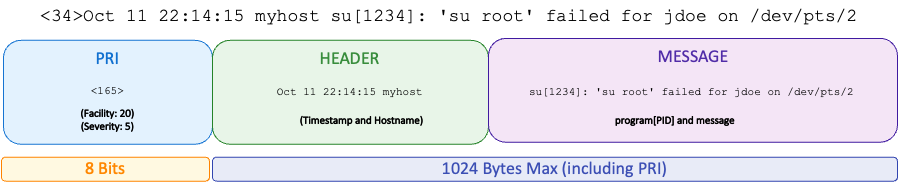
\includegraphics[width=0.8\textwidth]{Figuras/rfc3164.png}
    \caption{Estructura de un mensaje RFC 3164}
    \label{fig:rfc3164}
\end{figure}

La siguiente tabla describe los campos que componen un mensaje Syslog bajo este estandar.

\begin{longtable}{p{3cm} p{3cm} p{10cm}}
    \caption{Campos de un mensaje Syslog según RFC 3164}
    \label{tab:campos-rfc3164} \\

    \toprule
    \textbf{Campo} & \textbf{Valor} & \textbf{Descripción} \\
    \midrule
    \endfirsthead

    \multicolumn{3}{c}{\textit{Tabla \thetable. Continuación}} \\
    \toprule
    \textbf{Campo} & \textbf{Valor} & \textbf{Descripción} \\
    \midrule
    \endhead

    \midrule
    \multicolumn{3}{r}{\textit{Continúa en la siguiente página}} \\
    \endfoot

    \bottomrule
    \endlastfoot

    \texttt{PRI} &
    \texttt{<34>} &
    Indica la prioridad del mensaje y está compuesto por los valores de Facility y Severity. \\

    \texttt{TIMESTAMP} &
    \texttt{Oct 11 22:14:15} &
    Indica la fecha y hora en que se generó el evento. Utiliza el formato de mes, día, hora, minutos y segundos. \\

    \texttt{HOSTNAME} &
    \texttt{myhost} &
    Identifica el sistema o dispositivo que originó el mensaje. \\

    \texttt{TAG} &
    \texttt{su} &
    Permite identificar la aplicación o proceso asociado con la generación del mensaje. \\

    \texttt{PID} &
    \texttt{[1234]} &
    Identifica el proceso que generó el evento cuando el sistema emisor proporciona esta información. \\

    \texttt{MSG} &
    \texttt{'su root' failed for jdoe on /dev/pts/2} &
    Contiene la información específica del evento generado por la aplicación o dispositivo. \\

\end{longtable}

Una característica importante de RFC 3164 es que no define un esquema rígido para el contenido del campo MSG. El significado y formato de esta parte depende de la aplicación o dispositivo que genera el evento. Esto permite una gran flexibilidad, pero también introduce variabilidad entre fabricantes y sistemas.

A nivel de transporte, RFC 3164 contempla principalmente el uso de UDP, particularmente sobre el puerto 514, sin establecer mecanismos propios de confirmación, retransmisión o control de congestión. Por esta razón, el transporte definido bajo este modelo es de naturaleza no orientada a conexión y no garantiza la entrega de los mensajes.

Su diseño sencillo puede presentar dificultades en los entornos informáticos modernos. Por ejemplo, su formato de marca de tiempo carece de año y zona horaria, lo que puede generar confusión al correlacionar registros entre sistemas o durante investigaciones que abarcan varios periodos de tiempo. Actualente este estandar esta considerado como obsoleto y fue reemplazado formalmente por el estándar más completo RFC 5424, aunque sigue activo en algunos equipos y redes pequeñas.

\subsubsection{RFC 5424}
El RFC 5424, denominado The Syslog Protocol, fue publicado por el IETF en marzo de 2009, define un formato estandarizado para los mensajes del protocolo syslog \cite{rfc5424}. Su principal objetivo es proporcionar una estructura más precisa y extensible que la definida previamente por RFC 3164, algunas de las mejoras introducidas que buscan abordar las limitaciones son las siguientes:

\begin{itemize}
    \item RFC 5424 mejora considerablemente la representación temporal de los mensajes al incluir el año, la zona horaria y la posibilidad de registrar fracciones de segundo. Esto permite una mayor precisión en la marca temporal y facilita la correlación de eventos entre sistemas distribuidos.
    \item Introduce el campo STRUCTURED-DATA, lo que permite incorporar información estructurada dentro del mensaje. Esto hace posible que información que antes tendría que estar embebida en texto libre pueda representarse explícitamente como atributos.
    \item RFC 5424 utiliza $"-"$ como NILVALUE, es decir, indica que un determinado campo no tiene valor disponible. Esto facilita la interpretación de los mensajes y permite una mayor consistencia en la representación de datos faltantes.
\end{itemize}


La estructura de un mensaje RFC 5424 puede representarse conceptualmente como:

\begin{figure}[H]
    \centering
    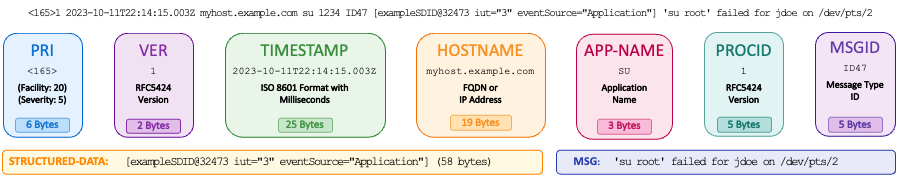
\includegraphics[width=1\textwidth]{Figuras/rfc5424.png}
    \caption{Estructura de un mensaje RFC 5424}
    \label{fig:rfc5424}
\end{figure}

La siguiente tabla describe los campos que componen un mensaje Syslog bajo este estandar.

\small
\begin{longtable}{p{3.0cm} p{2.0cm} p{10cm}}
    \caption{Campos del formato de mensaje Syslog definido en RFC 5424}
    \label{tab:rfc5424_fields} \\

    \toprule
    \textbf{Campo} & \textbf{Longitud} & \textbf{Descripción} \\
    \midrule
    \endfirsthead

    \multicolumn{3}{c}{\textit{Tabla \thetable. Continuación}} \\
    \toprule
    \textbf{Campo} & \textbf{Longitud} & \textbf{Descripción} \\
    \midrule
    \endhead

    \midrule
    \multicolumn{3}{r}{\textit{Continúa en la siguiente página}} \\
    \endfoot

    \bottomrule
    \endlastfoot

    \texttt{PRI} &
    1--3 caracteres &
    Contiene la prioridad del mensaje, calculada a partir de los valores de
    \textit{Facility} y \textit{Severity}. Se representa mediante un valor
    numérico encerrado entre los caracteres ``\texttt{<}'' y ``\texttt{>}''. \\

    \texttt{VERSION} &
    1--3 caracteres &
    Indica la versión del formato de mensaje Syslog utilizado. Para RFC 5424,
    el valor definido actualmente es \texttt{1}. \\

    \texttt{TIMESTAMP} &
    Variable &
    Indica la fecha y hora en la que se generó el evento. Utiliza un formato
    basado en ISO 8601 e incluye información de zona horaria y,
    opcionalmente, fracciones de segundo. \\

    \texttt{HOSTNAME} &
    Variable &
    Identifica el dispositivo o sistema que originó el mensaje. Puede
    corresponder al nombre de host, nombre de dominio o dirección IP del
    emisor, dependiendo de la información disponible. \\

    \texttt{APP-NAME} &
    1--48 caracteres &
    Identifica la aplicación o proceso que originó el mensaje. Permite asociar
    el evento con un componente específico del sistema emisor. \\

    \texttt{PROCID} &
    1--128 caracteres &
    Identifica el proceso que generó el mensaje. En sistemas donde sea
    aplicable, puede corresponder al identificador de proceso (PID). \\

    \texttt{MSGID} &
    1--32 caracteres &
    Identifica de forma única el tipo o clase de mensaje dentro del contexto
    de la aplicación que lo genera. Facilita la clasificación y correlación
    de eventos. \\

    \texttt{STRUCTURED-DATA} &
    Variable &
    Contiene información estructurada asociada al evento. Está formada por
    uno o más elementos de datos estructurados que pueden incluir parámetros
    con nombre y valor, facilitando el procesamiento automático de los
    mensajes. \\

    \texttt{MSG} &
    Variable &
    Contiene el contenido específico del evento. Puede incluir información
    adicional generada por la aplicación y, a diferencia de
    \textit{STRUCTURED-DATA}, generalmente se presenta como texto libre.

\end{longtable}

En cuanto a la longitud de los mensajes RFC 5424 no establece un límite máximo universal, el límite depende del transporte utilizado. Sin embargo, cualquier receptor debe poder aceptar mensajes de al menos 480 bytes y se recomienda que pueda aceptar hasta 2048 bytes.

Esto es relevante al trabajar con equipos de red porque algunos fabricantes generan mensajes considerablemente largos, especialmente cuando incluyen información estructurada o detalles adicionales del evento.

Finalmente, RFC 5424 define un mecanismo de transporte más flexible y confiable, permitiendo el uso de protocolos orientados a conexión como TCP y TLS, además del tradicional UDP. Estas especificaciones estan descritas en el RFC 5425 (TLS) \cite{rfc5425} y RFC 5426 (TCP) \cite{rfc5426}.

\section{Syslog-ng}
Syslog-ng es una aplicación de gestión de registros diseñada para la recopilación, procesamiento y distribución centralizada de mensajes de log. Su arquitectura permite recibir información proveniente de diferentes fuentes, aplicar operaciones de filtrado, análisis y transformación, y posteriormente enviar los mensajes procesados hacia uno o varios destinos.

Una de las principales características es su capacidad para trabajar con una gran variedad de fuentes y destinos. El proyecto soporta mecanismos de entrada y salida asociados con Syslog, texto no estructurado, colas de mensajes, bases de datos SQL y NoSQL y plataformas de procesamiento de grandes volúmenes de información. También dispone de integraciones con tecnologías como Elasticsearch, Apache Kafka y Hadoop.

La Open Source Edition (OSE) de syslog-ng es un proyecto de código abierto cuyo código fuente se encuentra disponible públicamente. El proyecto utiliza las licencias GNU General Public License (GPL) y GNU Lesser General Public License (LGPL), dependiendo del componente. La comunidad mantiene el código, documentación, correcciones y nuevas funcionalidades mediante un modelo de desarrollo abierto \cite{syslogng_community}.

\subsection{Arquitectura y procesamiento}
El funcionamiento de syslog-ng se basa en varios objetos de configuración que definen cómo deben ser recibidos y procesados los mensajes. Los principales componentes son sources, destinations, filters, parsers, rewrite rules, templates y log paths \cite{syslogng_documentation}.
\begin{equation}
\boxed{
\substack{\text{Fuente de}\\\text{eventos}}
\rightarrow
\substack{\text{SOURCE}\\\text{Recepción}}
\rightarrow
\substack{\text{FILTER / PARSER}\\\text{Clasificación y extracción}}
\rightarrow
\substack{\text{REWRITE}\\\text{Normalización}}
\rightarrow
\substack{\text{TEMPLATE}\\\text{Formateo}}
\rightarrow
\substack{\text{DESTINATION}\\\text{Entrega}}
}
\label{eq:flujo-syslog-ng}
\end{equation}

El funcionamiento de cada uno es el siguiente:

\subsubsection{Sources}
Representan los puntos de entrada de los mensajes
hacia syslog-ng. Mediante este componente se define el mecanismo utilizado para recibir los registros generados por dispositivos, aplicaciones o sistemas externos.

Entre las fuentes disponibles se encuentran los archivos locales, los
sockets del sistema y las conexiones de red mediante protocolos como UDP y TCP.

Un ejemplo de una fuente de red que recibe mensajes mediante UDP en el
puerto 514 es:

\begin{lstlisting}[style=logstyle]
source s_network {
    network(
        ip(0.0.0.0)
        port(514)
        transport("udp")
    );
};
\end{lstlisting}

En este caso, \texttt{s\_network} identifica la fuente y el controlador
\texttt{network} establece las características de la recepción de los
mensajes.

\subsubsection{Filters}
Los filtros permiten seleccionar los mensajes que cumplen
determinadas condiciones. Estas condiciones pueden estar relacionadas con campos del mensaje Syslog, como facility, severity, host de origen, aplicación o contenido del mensaje.

Por ejemplo, es posible crear un filtro para seleccionar únicamente mensajes relacionados con autenticación:

\begin{lstlisting}[style=logstyle]
filter f_auth {
    facility(auth);
};
\end{lstlisting}

Los filtros pueden combinarse mediante operadores lógicos para construir condiciones más específicas. Esto permite separar los eventos según su naturaleza antes de enviarlos hacia los destinos correspondientes.

\subsubsection{Parsers}
Permiten analizar el contenido de los mensajes y
extraer información estructurada. Esta funcionalidad es especialmente importante cuando los dispositivos utilizan formatos propios o cuando la información relevante se encuentra dentro del campo de mensaje como por ejemplo:

\begin{lstlisting}[style=logstyle]
user=jdoe src=192.168.1.25 action=login status=failed
\end{lstlisting}

puede ser procesado para obtener diferentes campos:

\begin{lstlisting}[style=logstyle]
user   = jdoe
src    = 192.168.1.25
action = login
status = failed
\end{lstlisting}

Luego la informacion extraida se usa con mayor facilidad en filtros, reescrituras y plantillas.

\subsubsection{Rewrite}

Permiten modificar los valores asociados a un mensaje durante su procesamiento. Pueden utilizarse para reemplazar,
eliminar o establecer valores con el objetivo de normalizar la información proveniente de diferentes fuentes, como por ejemplo cuando diferentes dispositivos representan un mismo evento mediante expresiones diferentes:

\begin{lstlisting}[style=logstyle]
Login failed
Authentication failure
AUTH_FAIL
\end{lstlisting}

Mediante reglas de reescritura, estos valores pueden transformarse en una representación común:

\begin{lstlisting}[style=logstyle]
event_type=authentication_failure
\end{lstlisting}

Esta capacidad es muy fuerte en infraestructuras heterogéneas, ya que permite establecer una representación uniforme antes de entregar los eventos a una plataforma de análisis.

\subsubsection{Templates}
Definen la representación final de los mensajes
que serán enviados a un destino. Estas utilizan macros y valores estructurados disponibles durante el procesamiento para construir el contenido de salida.

Por ejemplo, puede definirse una plantilla para generar una estructura JSON:

\begin{lstlisting}[style=logstyle]
template t_json {
    template("{\"host\":\"${HOST}\",
\"program\":\"${PROGRAM}\",
\"message\":\"${MESSAGE}\"}\n");
};
\end{lstlisting}

Las plantillas permiten adaptar el formato de los registros a los requerimientos del sistema que los recibe.

\subsubsection{Destinations}

Representan los puntos hacia los cuales syslog-ng entrega los mensajes después de su procesamiento. Un destino puede corresponder a un archivo local, una base de datos, un servicio remoto o un dispositivo externo.

Por ejemplo, para almacenar los mensajes en un archivo:

\begin{lstlisting}[style=logstyle]
destination d_logs {
    file("/var/log/network.log");
};
\end{lstlisting}

Y para configurarse un destino de red para reenviar los mensajes hacia otro servidor:

\begin{lstlisting}[style=logstyle]
destination d_wazuh {
    network(
        "192.168.1.100"
        port(514)
        transport("udp")
    );
};
\end{lstlisting}

En la arquitectura implementada en el proyecto, este mecanismo permite utilizar syslog-ng como intermediario entre los dispositivos que generan los registros y la plataforma Wazuh.

\subsubsection{Log paths}
Definen las rutas de procesamiento que siguen los mensajes dentro de syslog-ng. En ellos se relacionan las fuentes, filtros, procesadores y destinos, estableciendo de esta manera el flujo de los registros:

\begin{lstlisting}[style=logstyle]
log {
    source(s_network);
    filter(f_auth);
    destination(d_wazuh);
};
\end{lstlisting}

En este caso, los mensajes recibidos mediante \texttt{s\_network} son evaluados por el filtro \texttt{f\_auth}. Aquellos que cumplen la condición establecida son enviados posteriormente hacia \texttt{d\_wazuh}.

Los log paths constituyen, por tanto, el mecanismo mediante el cual los diferentes componentes de syslog-ng se integran para construir el flujo de procesamiento de los registros.

\section{Sistemas de Gestión de Información y Eventos de Seguridad (SIEM)}
\section{Wazuh}
\section{Correlación de eventos}
\section{Detección y respuesta ante incidentes}
\chapter{CONTEXTO DEL PROYECTO}

\section{Contexto empresarial}
EMCALI EICE ESP es una empresa de servicios públicos que desarrolla actividades asociadas a diferentes áreas de prestación de servicios a la comunidad. Dentro de su estructura se encuentra la Unidad de Gestión de Plataformas de Servicios y Contenidos (UGPSC), encargada de la operación y administración de la infraestructura que soporta los servicios de telecomunicaciones ofrecidos por la organización.

El presente proyecto de práctica profesional se desarrolla específicamente en el contexto de esta unidad y se encuentra orientado a la gestión y análisis de los registros generados por las plataformas y dispositivos que hacen parte de su infraestructura. Por lo tanto, el alcance del proyecto se encuentra directamente relacionado con los servicios de Internet, televisión sobre IP (IPTV) y voz sobre IP (VoIP).

La infraestructura asociada a estos servicios comprende diferentes elementos de acceso, agregación y transporte, cuya operación requiere ser supervisada para identificar oportunamente eventos relacionados con su funcionamiento y particularmente, con aspectos asociados a la seguridad de la infraestructura tecnológica.

\section{Diversidad de la infraestructura tecnológica}
La red administrada por la UGPSC se encuentra conformada por equipos de diferentes fabricantes, entre los que se encuentran Juniper, Huawei, Cisco, HP, FiberHome y Fortinet. Esta heterogeneidad constituye un factor relevante para la gestión de los registros, debido a que cada fabricante usa formatos diferentes para la información de sus eventos.

La infraestructura también comprende servidores que participan en la prestación y administración de los servicios de telecomunicaciones. Por esta razón, el proyecto no se limita exclusivamente a los registros provenientes de los equipos de red, sino que contempla también aquellos generados por dichos servidores.

\section{Situación inicial del ISP}
Antes del desarrollo del proyecto, los registros generados por los diferentes dispositivos de la infraestructura eran centralizados en un servidor syslog-ng. Sin embargo, la plataforma utilizada contaba con una versión antigua y los registros eran almacenados de manera masiva y sin un proceso de organización o clasificación que facilitara su análisis cuando hubiesen fallos o incidentes.

Como consecuencia, cuando esto pasaba o se requería verificar el comportamiento registrado por un dispositivo, el proceso de consulta implicaba realizar búsquedas y filtros directamente sobre grandes cantidades de registros almacenados en el servidor. Esta situación dificultaba la identificación de información relevante, especialmente cuando era necesario analizar acontecimientos ocurridos durante un periodo determinado o relacionar registros generados por diferentes dispositivos.

El problema no estaba relacionado solamente con la cantidad de información almacenada. La heterogeneidad de los dispositivos también implicaba que los registros presentaran diferentes estructuras y formatos, lo que dificultaba su comparación, por lo tanto, aunque la infraestructura dispusiera de una fuente centralizada de registros, no había un mecanismo especializado que transformara ese volumen de información en eventos de seguridad fácilmente identificables y que estuviesen organizados por fabricante o etapa de la red.

\section{Antecedentes y propósito del proyecto}
Como antecedente del proyecto, un ingeniero que se incorporó a la UGPSC había desarrollado una implementación basada en Graylog para el procesamiento de registros provenientes de un equipo de red Huawei. Esta solución permitía extraer información relevante de los registros y generar alertas asociadas a determinados parámetros de operación del dispositivo. Esta experiencia permitió identificar el potencial del procesamiento centralizado de registros como mecanismo para obtener información relevante a partir de los eventos generados por la infraestructura.

El proyecto se planteó como una solución complementaria a las herramientas de monitoreo operativo existentes, particularmente Zabbix, utilizado para la supervisión de variables de operación, rendimiento y disponibilidad mediante SNMP. En contraste, la solución desarrollada se orienta al análisis de los eventos registrados desde una perspectiva de ciberseguridad, considerando información de autenticaciones, cambios de configuración, fallos, accesos, establecimiento y terminación de sesiones y otros eventos que pueden adquirir relevancia al ser analizados de manera conjunta.

Dentro del alcance de la práctica se encuentra la configuración y administración de ambas plataformas, así como el desarrollo y ajuste continuo de reglas, decoders y mecanismos de procesamiento. Asi, el proyecto no se limita a la implementación de una plataforma de monitoreo, sino que comprende un proceso de investigación, desarrollo y optimización de mecanismos de detección orientados a las características particulares del ISP.
\chapter{OBJETIVOS}

\section{Objetivo general}
Implementar una solución de gestión de eventos e información de seguridad (SIEM) basada en Wazuh para la recolección, normalización, análisis y correlación centralizada de eventos provenientes de dispositivos y sistemas de la infraestructura de telecomunicaciones.

\section{Objetivos específicos}
\begin{enumerate}
    \item Establecer un servidor centralizado para la recolección y procesamiento de los logs generados por los diferentes dispositivos de la RMS.
    \item Caracterizar y normalizar los eventos recolectados, identificando las principales estructuras y tipos de información presentes en los registros para facilitar su posterior procesamiento.
    \item Implementar mecanismos de análisis y correlación de eventos mediante Wazuh, orientados a la identificación de patrones y comportamientos asociados con incidentes o situaciones relevantes para la seguridad de la infraestructura.
    \item Diseñar y ajustar reglas de detección y generación de alertas, de acuerdo con los eventos y escenarios identificados buscando mejorar progresivamente la capacidad de detección de la solución.
    \item Implementar mecanismos de visualización y monitoreo mediante dashboards y reportes, que permitan monitorear de manera clara e interpretable los eventos, alertas y principales indicadores obtenidos a partir de la información procesada.
\end{enumerate}
%\begin{table}[H]
\captionsetup{justification=raggedright,singlelinecheck=false}
\caption{Cronograma de actividades}
\small
\setlength{\tabcolsep}{2pt}
\begin{tabular}{cc|llll|llll|llll|llll|llll|llll|llll|llll|llll|}
\cline{3-38}
\multicolumn{2}{l|}{} & \multicolumn{4}{c|}{\cellcolor[HTML]{FFCE93}MES 1} & \multicolumn{4}{c|}{\cellcolor[HTML]{FFCE93}MES 2} & \multicolumn{4}{c|}{\cellcolor[HTML]{FFCE93}MES 3} & \multicolumn{4}{c|}{\cellcolor[HTML]{FFCE93}MES 4} & \multicolumn{4}{c|}{\cellcolor[HTML]{FFCE93}MES 5} & \multicolumn{4}{c|}{\cellcolor[HTML]{FFCE93}MES 6} & \multicolumn{4}{c|}{\cellcolor[HTML]{FFCE93}MES 7} & \multicolumn{4}{c|}{\cellcolor[HTML]{FFCE93}MES 8} & \multicolumn{4}{c|}{\cellcolor[HTML]{FFCE93}MES 9} \\ \hline
\rowcolor[HTML]{FFCE93} 
\multicolumn{1}{|c|}{\cellcolor[HTML]{FFCE93}ETAPA} & ACTIVIDAD & \multicolumn{1}{c|}{\cellcolor[HTML]{FFCE93}1} & \multicolumn{1}{c|}{\cellcolor[HTML]{FFCE93}2} & \multicolumn{1}{c|}{\cellcolor[HTML]{FFCE93}3} & \multicolumn{1}{c|}{\cellcolor[HTML]{FFCE93}4} & \multicolumn{1}{c|}{\cellcolor[HTML]{FFCE93}1} & \multicolumn{1}{c|}{\cellcolor[HTML]{FFCE93}2} & \multicolumn{1}{c|}{\cellcolor[HTML]{FFCE93}3} & \multicolumn{1}{c|}{\cellcolor[HTML]{FFCE93}4} & \multicolumn{1}{c|}{\cellcolor[HTML]{FFCE93}1} & \multicolumn{1}{c|}{\cellcolor[HTML]{FFCE93}2} & \multicolumn{1}{c|}{\cellcolor[HTML]{FFCE93}3} & \multicolumn{1}{c|}{\cellcolor[HTML]{FFCE93}4} & \multicolumn{1}{c|}{\cellcolor[HTML]{FFCE93}1} & \multicolumn{1}{c|}{\cellcolor[HTML]{FFCE93}2} & \multicolumn{1}{c|}{\cellcolor[HTML]{FFCE93}3} & \multicolumn{1}{c|}{\cellcolor[HTML]{FFCE93}4} & \multicolumn{1}{c|}{\cellcolor[HTML]{FFCE93}1} & \multicolumn{1}{c|}{\cellcolor[HTML]{FFCE93}2} & \multicolumn{1}{c|}{\cellcolor[HTML]{FFCE93}3} & \multicolumn{1}{c|}{\cellcolor[HTML]{FFCE93}4} & \multicolumn{1}{c|}{\cellcolor[HTML]{FFCE93}1} & \multicolumn{1}{c|}{\cellcolor[HTML]{FFCE93}2} & \multicolumn{1}{c|}{\cellcolor[HTML]{FFCE93}3} & \multicolumn{1}{c|}{\cellcolor[HTML]{FFCE93}4} & \multicolumn{1}{c|}{\cellcolor[HTML]{FFCE93}1} & \multicolumn{1}{c|}{\cellcolor[HTML]{FFCE93}2} & \multicolumn{1}{c|}{\cellcolor[HTML]{FFCE93}3} & \multicolumn{1}{c|}{\cellcolor[HTML]{FFCE93}4} & \multicolumn{1}{c|}{\cellcolor[HTML]{FFCE93}1} & \multicolumn{1}{c|}{\cellcolor[HTML]{FFCE93}2} & \multicolumn{1}{c|}{\cellcolor[HTML]{FFCE93}3} & \multicolumn{1}{c|}{\cellcolor[HTML]{FFCE93}4} & \multicolumn{1}{c|}{\cellcolor[HTML]{FFCE93}1} & \multicolumn{1}{c|}{\cellcolor[HTML]{FFCE93}2} & \multicolumn{1}{c|}{\cellcolor[HTML]{FFCE93}3} & \multicolumn{1}{c|}{\cellcolor[HTML]{FFCE93}4} \\ \hline
\multicolumn{1}{|c|}{\cellcolor[HTML]{FFCE93}} & \cellcolor[HTML]{FFCE93}Actividad I & \cellcolor[HTML]{FFFE65} & \cellcolor[HTML]{FFFE65} & \cellcolor[HTML]{FFFE65}{\color[HTML]{FFFC9E} } & \cellcolor[HTML]{FFFE65} & \cellcolor[HTML]{FFFE65} &  &  &  &  &  &  &  &  &  &  &  &  &  &  &  &  &  &  &  &  &  &  &  &  &  &  &  &  &  &  &  \\ \cline{2-38} 
\multicolumn{1}{|c|}{\cellcolor[HTML]{FFCE93}} & \cellcolor[HTML]{FFCE93}Actividad II &  &  &  &  &  & \cellcolor[HTML]{FFFE65} & \cellcolor[HTML]{FFFE65} &  &  &  &  &  &  &  &  &  &  &  &  &  &  &  &  &  &  &  &  &  &  &  &  &  &  &  &  &  \\ \cline{2-38} 
\multicolumn{1}{|c|}{\multirow{-3}{*}{\cellcolor[HTML]{FFCE93}ETAPA I}} & \cellcolor[HTML]{FFCE93}Actividad III &  &  &  &  &  &  &  & \cellcolor[HTML]{FFFE65} & \cellcolor[HTML]{FFFE65} &  &  &  &  &  &  &  &  &  &  &  &  &  &  &  &  &  &  &  &  &  &  &  &  &  &  &  \\ \hline
\multicolumn{1}{|c|}{\cellcolor[HTML]{FFCE93}} & \cellcolor[HTML]{FFCE93}Actividad IV &  &  &  &  &  &  &  &  &  & \cellcolor[HTML]{6200C9} & \cellcolor[HTML]{6200C9} & \cellcolor[HTML]{6200C9} & \cellcolor[HTML]{6200C9} &  &  &  &  &  &  &  &  &  &  &  &  &  &  &  &  &  &  &  &  &  &  &  \\ \cline{2-38} 
\multicolumn{1}{|c|}{\cellcolor[HTML]{FFCE93}} & \cellcolor[HTML]{FFCE93}Actividad V &  &  &  &  &  &  &  &  &  &  &  &  &  & \cellcolor[HTML]{6200C9} & \cellcolor[HTML]{6200C9} & \cellcolor[HTML]{6200C9} &  &  &  &  &  &  &  &  &  &  &  &  &  &  &  &  &  &  &  &  \\ \cline{2-38} 
\multicolumn{1}{|c|}{\multirow{-3}{*}{\cellcolor[HTML]{FFCE93}ETAPA II}} & \cellcolor[HTML]{FFCE93}Actividad VI &  &  &  &  &  &  &  &  &  &  &  &  &  &  &  &  & \cellcolor[HTML]{6200C9} & \cellcolor[HTML]{6200C9} &  &  &  &  &  &  &  &  &  &  &  &  &  &  &  &  &  &  \\ \hline
\multicolumn{1}{|c|}{\cellcolor[HTML]{FFCE93}} & \cellcolor[HTML]{FFCE93}Actividad VII &  &  &  &  &  &  &  &  &  &  &  &  &  &  &  &  &  &  & \cellcolor[HTML]{32CB00} & \cellcolor[HTML]{32CB00} & \cellcolor[HTML]{32CB00} & \cellcolor[HTML]{32CB00} &  &  &  &  &  &  &  &  &  &  &  &  &  &  \\ \cline{2-38} 
\multicolumn{1}{|c|}{\cellcolor[HTML]{FFCE93}} & \cellcolor[HTML]{FFCE93}Actividad VIII &  &  &  &  &  &  &  &  &  &  &  &  &  &  &  &  &  &  &  &  &  &  & \cellcolor[HTML]{32CB00} & \cellcolor[HTML]{32CB00} & \cellcolor[HTML]{32CB00} & \cellcolor[HTML]{32CB00} &  &  &  &  &  &  &  &  &  &  \\ \cline{2-38} 
\multicolumn{1}{|c|}{\multirow{-3}{*}{\cellcolor[HTML]{FFCE93}ETAPA III}} & \cellcolor[HTML]{FFCE93}Actividad IX &  &  &  &  &  &  &  &  &  &  &  &  &  &  &  &  &  &  &  &  &  &  &  &  &  &  & \cellcolor[HTML]{32CB00} & \cellcolor[HTML]{32CB00} &  &  &  &  &  &  &  &  \\ \hline
\multicolumn{1}{|c|}{\cellcolor[HTML]{FFCE93}} & \cellcolor[HTML]{FFCE93}Actividad X &  &  & \cellcolor[HTML]{00D2CB} &  & \cellcolor[HTML]{00D2CB} &  & \cellcolor[HTML]{00D2CB} &  & \cellcolor[HTML]{00D2CB} &  & \cellcolor[HTML]{00D2CB} &  & \cellcolor[HTML]{00D2CB} &  & \cellcolor[HTML]{00D2CB} &  & \cellcolor[HTML]{00D2CB} &  & \cellcolor[HTML]{00D2CB} &  & \cellcolor[HTML]{00D2CB} &  & \cellcolor[HTML]{00D2CB} &  & \cellcolor[HTML]{00D2CB} &  & \cellcolor[HTML]{00D2CB} &  & \cellcolor[HTML]{00D2CB} & \cellcolor[HTML]{00D2CB} & \cellcolor[HTML]{00D2CB} & \cellcolor[HTML]{00D2CB} &  &  &  &  \\ \cline{2-38} 
\multicolumn{1}{|c|}{\cellcolor[HTML]{FFCE93}} & \cellcolor[HTML]{FFCE93}Actividad XI &  &  &  &  &  &  &  &  &  &  &  &  &  &  &  &  &  &  &  &  &  &  &  &  &  &  &  &  &  &  & \cellcolor[HTML]{00D2CB} & \cellcolor[HTML]{00D2CB} &  &  &  &  \\ \cline{2-38} 
\multicolumn{1}{|c|}{\multirow{-3}{*}{\cellcolor[HTML]{FFCE93}ETAPA IV}} & \cellcolor[HTML]{FFCE93}Actividad XII &  &  &  &  &  &  &  &  &  &  &  &  &  &  &  &  &  &  &  &  &  &  &  &  &  &  &  &  &  &  &  &  & \cellcolor[HTML]{00D2CB} & \cellcolor[HTML]{00D2CB} & \cellcolor[HTML]{00D2CB} & \cellcolor[HTML]{00D2CB} \\ \hline
\end{tabular}
\end{table}


%%%%%%%%%%%%%%%%%%%%%%%%%%%%%%%%%%%%%%%%%%%%%%%%%%%%%%
% Seleccione un estilo para la bibliografía
%%%%%%%%%%%%%%%%%%%%%%%%%%%%%%%%%%%%%%%%%%%%%%%%%%%%%%%
\bibliographystyle{ieeetr}
%bibliographystyle{apalike}
%\bibliographystyle{abbrv}
%\bibliographystyle{acm}
%\bibliographystyle{alpha}
%\bibliographystyle{plain}
%\bibliographystyle{siam}
%\bibliographystyle{unsrt}

%%%%%%%%%%%%%%%%%%%%%%%%%%%%%%%%%%%%%%%%%%%%%%%%%%%%%%%
\phantomsection
%\addcontentsline{toc}{chapter}{REFERENCIAS}
\renewcommand{\bibname}{{\normalsize\rm \textbf{REFERENCIAS}}}
\vspace{-1.5cm}
% Defina el archivo .bib con sus referencias
\footnotesize{
\bibliography{Referencias/references}
}
%\end{document}

%%%%%%%%%%%%%%%%%%%%%%%%%%%%%%%%%%%%%%%%%%%%%%%%%%%%%%%%
% En caso de necesitar agregar apéndices, habilite el siguiente comando.
%\include{data/appendices}
%\appendix
%\input{data/apendice2.tex}
\end{document}
